\chapter{A Theory of Influences on Security Practices}\label{C:Emergent Theory}

This chapter will outline the emergent theory. \textbf{The three-step coding process }s described in the methodology section was used to achieve this theory. The three found categories and the relationship between each of them will be further explained.

\subsection{Emergent Theory}

The emergent theory consists of three main categories on what influence programmers:

\begin{enumerate}
\item  Culture in groups of individuals
\item Organisational structure and practices
\item Industry trends
\end{enumerate}

\begin{figure}[ht]
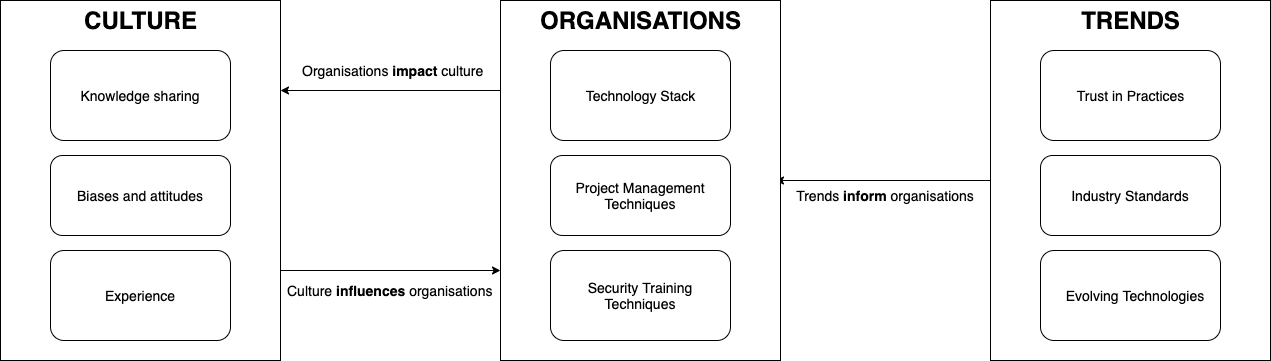
\includegraphics[width=17cm]{figures/fig2.png}
\centering
\caption{The Theory of Influences on Security Practices}
\centering
\end{figure}

\section{Culture}

This category is the effect of the culture we see in groups of individuals. The term culture refers to the customs that programmers have in order to maintain security: knowledge sharing, biases and attitudes and experience. 

\subsection{Knowledge Sharing}

Knowledge sharing is deliberate exchange of information and it was highly regarded among the participants \cite{know}. Participants identified communication between team-mates as being a key way to learn and better current and new security practices. These opportunities are taken within teams and are often done when peer-programming or simply asking questions. 
\newline
\par
\textit{"I like that people come to me when they need help. I think that is the best way for everyone to learn, even me!" - P3}
\newline
\par
Often vital knowledge sharing moments happened in passing. When programmers were stuck with using a library, framework or even learning a newer language nuance, they appreciated the ability to turn to the person next to them and get help. 
\newline
\par \textit{"...we've got a really flat structure, if I needed to I could pretty much directly ping someone..." - P10 }
\newline
\par
Participant \textit{[P8]} defined that the open communication streams between people across business and experiences made it easier to obtain answers. Walking between desks to other teams and also sending anyone emails regardless of hierarchy helped facilitate these exchanges. These exchanges were often more attainable in smaller organisations where individuals were more familiar \textit{{P5, P8, P9}}. 
\newline
\par 
\textit{"It's a lot easier when there are only seven people in my company. - P8"}
\newline
\par
This is harder to maintain in larger organisations. 
\newline
\par
\textit{"You don't do technical inductions which is quite irritating  because you do have to know people and you do have to  find people who know stuff - P11"}
\newline
\par
\textit{"I think bigger companies have very secure processes, and it's very need-to-know and there is a very clear divide and no one is afraid to say that it's above your clearance. Smaller companies the lines are a little bit blurred on clearance... I think [at] the size of that is find because there is communication... I think security is far more approachable in a smaller company; it seems far more reasonable and accessible." - P8}

\subsection{Biases and attitudes}

\par Participants had very strong preferences to how security practices aligned with their work. Those who were strictly developers \textit{[P4, P5, P7]} typically found it a deterrence to completing their work on time, while the others had more of a positive attitude towards managing security. 
\newline
\par 
\textit{"I believe that tasks kind of [get] pushed back a month or two purely because security teams get quite busy on an ad-hoc basis and hiding something, removing something, [adding something], can understandably be a bigger thing, even if it is one manager asking for access... Now we are aware of the leak times that those kind of security tasks can take and so we do plan for those, but I'll also probably say a lot of those times we don't plan enough" - P7}
\newline
\par
\textit{"... It is going to take time, my point was we can manage it nicely without confusing people" - P1}
\newline
\par
This also showed that often, people had a more positive demeanour when dealing with technologies based on familiarity. 
\newline
\par \textit{"... when a change happens that they don't like, there have been people who have straight up left and quit their jobs... their empire is DESTROYED!"  - P11}
\newline
\par
\textit{"For me, I know that it is important so I'm willing to compromise on that on a personal level, but I can get where that someone that it is not their, not their thing, they can see it as a hindrance"  - P12}
\newline
\par One participant \textit{[P11]} acknowledged the personal relationships within the workplace as contributing to biases in the \textit{"tech bro-culture" }. They gave the example of a vendor-client relationship that they had witnessed where the vendor accepted any requests into production because of the close friendship with the client. The client had not given any comments and had caused the build pipeline to fail many times and it was still was not working as the vendor continued to approve changes. This \textit{"tech bro-culture"} also exhibits explicit favouritism between small groups of people in an organisation. People also have a view where asking questions makes you seem lesser than, and therefore, there was a cultivated culture on this lack-of-communication. They stated that a lot of the time in this industry people would say that they know something when they do not. 

\subsection{Experience}

\par Experience pertains to the level of expertise an individual has in the industry. This was not only measured by the amount of years that they have worked, but also whether they have worked on a range of projects. One participant \textit{[P11]} is an example of this; have only worked 2-5 years in industry, but have worked in multiple government and private organisations during this time. They regularly advise the seniors in their team on the work that they do as their experiences are related to their background in the industry.
\newline
\par
\textit{"... Which is a strange dynamic because they're both seniors... Yeah, I'm a lot younger, I'm the only woman and I have a lot more experience than they do in the specific stuff that we're working in right now. And a lot of where my skill-set comes in is like picking up things up quickly because I have moved around a lot, I have done a whole bunch of random stuff".}
\newline
\par
Almost all the participants identified major differences in how less experienced and more experienced individuals deal with security practices. Often less experienced team members are wanting and willing to learn, but still are lacking in the ability to identify key threats and risks which a more experienced team member is more versed in doing. 
\newline
\par
\textit{"New team members, I find, that they're kinda charged-up, ready-to-go, and that they want to prove themselves. I do find the more experienced people are a little more humble and they're a little bit more set-back... it's a bit more of a  different energy-vibe; you see the new people come in, so ready to learn and they want to do security and then you get the people who have been there for ages like oh yeah that's easy and just do it." - P6 }
\newline
\par
\textit{"I am relatively new to the industry so I come in with a fresh mind. " -P5}

\section{Organisations}

This category presents the influence of organisational practices and structuring of security practices. The attributes within this category are the parts of an organisation which motivated programmer choices: technology stack, project management techniques and security training techniques. 

\subsection{Technology Stack}

\par The technology stack is the security tools, frameworks, libraries and languages in use in an organisation. Throughout the study it was prevalent that organisations have existing security programming languages that they use. 
\newline
\par
\textit{"I'd say company-wide [language]... Java for the back-end using spring as the framework and JavaScript for the front-end using React as the framework." - P5}
\newline
\par
\textit{"We go with C\# and React JavaScript because those are the languages more-or-less used around the company" - P7}
\newline
\par
\textit{"We are a Microsoft technology stack company so we are very much on C\#, and so Microsoft C\#, and [the] legacy system has Visual, VB.net" - P13}
\newline
\par
These are chosen based on legacy technologies already in use [P13] and legacy products that organisations provide clients [P3, P7].  Not a lot flexibility is given to programmers to choose language and if they try lobby a change there is a very long term process in approving \textit{[P10]} which dissuade them in trying to make any changes to the current process.
\newline
\par 
\textit{"If you make a request, you don't know when you're going to hear back, so that's one of the constraints... you can prioritise stuff and they can probably get it done, but for other stuff, like I'm trying to get a tool approved... I filled in a form in literally April, and security hasn't gotten back to me. It's kind of an example that security ignores you and you can't use a tool without approval." - P10}
\newline
\par
\textit{"If you ask questions a lot of the time your work gets halted... I don't know what they are doing because they certainly aren't listening to you or replying to your emails." - P11}
\newline
\par
When asked about whether languages changed dependent on security practices and/or requirements the answer was often,
\newline
\par \textit{"No." - P4}.
\newline
\par 
\textit{"I'd say security is not the biggest factor is choosing [a language]" - P7 }
\newline
\par
\textit{"I don't think it is the direct result of security, it's the result of functionality" - P8}
\newline
\par One participant did mention that their libraries and tools did not change based on the security needs as they use ones that can be used across languages [P13].
\newline
\par
\textit{"We haven't seen a library which is not compatible over many languages ... " - P13}
\newline
\par Two outliers that were able to change languages related to security. Both the cloud engineers \textit{[P11, P12]} stated that languages were changed based on their security needs; not on features or familiarity. Especially when working on the security of pipelines, but pipelines themselves were mandated by the organisation. 
\newline
\par
\textit{"...we picked this tool... we also couldn't pick our pipelining tool, that was Jenkins and that's a corporate mandate... I think what makes us different is that we deal with CI/CD so need to keep up-to-date and research more..." - P11}

\subsection{Project Management Techniques}

\par Project management techniques are set by the organisational structuring and choices of more senior people within companies. Participants indicated these project management techniques as effecting how they implemented security in their work. The three project management techniques mentioned in this section are Waterfall, Agile and DevOps. Waterfall is where a development team follows a linear movement in completing a project and any obstructions are not planned for \cite{water} . Agile methodology uses the idea of sprints to define breaking up the original brief into mini-goals \cite{water}. DevOps is the newest trend where instead of delivering a small output at the end of each sprint, there is continuous delivery \cite{ubiq}. Agile and DevOps can both use the idea of cross-functional teams to promote collaboration. 
\newline
\par 
One participant \textit{[P10]} used the Waterfall methodology, while other participants \textit{[P3, P4, P5, P7, P8, P11, P12, P13, P15]} worked with either Agile or DevOps project management. When managed correctly, the techniques benefited participants a lot. It was easier getting the security teams involved throughout the process in a more DevOps approach, and with an Agile approach each deliverable are checked at the end of each sprint, but strict management styles were not enforced. 
\newline
\par
\textit{"It is a major problem with the Waterfall type projects.... it's slowly going out, but very slowly, and they've left a lot of things behind, or rather forgotten to update a bunch of processes to match this stuff... Most places that I've worked, we do Agile, we do DevOps, but [also] not really. It's a whole thing." - P11}
\newline
\par
Traditional waterfall-type management leaks through and some participants felt as though there is an emphasis of security at the beginning and end of projects rather than throughout as a means to reduce \textit{"tech-debt" [P7]} which does the opposite as programmers then struggle to fix multiple issues at the end. 
\newline
\par 
\textit{"I think that it takes the load of developers so developers can just focus on building [a] good application. I think the set-up right now [by having a separate security team] is pretty good right now. I, I just say that it is just annoying putting the request through and them being slow" - P10}
\newline
\par 
Participants with more senior roles \textit{[P3, P4]} did not like the wave of DevOps management; it was identified as being too time consuming or just a fad. The feelings to do with security were different as one was a developer \textit{[P4]} and one was a security architect \textit{[P3]}. The latter critique also stemmed from a hatred of buzz-words when they mentioned DevSecOps; a more security specific iteration of DevOps project management.
\newline
\par \textit{"It's just annoying and gets in the way of my work" - P4}
\newline
\par \textit{"... I don't like it. No one actually follows anything anyway, and an ongoing security approach should be there already..." - P3}
\newline
\par 
The project management techniques also influenced how teams interacted with each other. With a DevOps approach, the support from the security team was continuous and talking between teams occurred more often. . Often a security person was fully involved in the entire project; consequently this increased collaboration meant that security issues were being identified earlier, not just near deadlines or after completion. 
\newline
\par 
\textit{"The cross-functional teams, is how I've kind of been told to refer to them; they're really good... Anyway the point was, yeah, a lot of it is around your organisational structure and the way you form your teams. It's a major problem with like waterfall-type projects where you do like dev, and then you do test and then you do security at the end, but that's, it's slowly going out, but I mean like very slowly, and they've left a lot of things behind, or rather forgotten to update a bunch of processes to match this sort of stuff." - P11}
\newline
\par
This does not often occur due to a lack of resources such as skilled employees and money as different business units charge for time \textit{[P12]}. 
\newline
\par
\textit{"Ideally that [would] be awesome, but you have to pay all those people." - P12 }

\subsection{Security Training Techniques}
\par 
Security training techniques and methods are chosen internally by the organisations. Participants \textit{[P1, P2, P3, P6, P7, P9, P10, P11, P12, P13, P14, P15]} state that they have not been exposed to much security training during their prior education so the training's that work provide are key in educating employers in how to protect assets and mitigate risks and are ongoing. 
\newline
\par 
\textit{"I don't have any formal education, but I have worked in security roles in two other organisations" - P2}
\newline
\par
\textit{"The closest thing really is [learning about] concurrency [at uni] for the most part." - P5}
\newline
\par
\textit{"I had one security paper when I was studying" - P6}
\newline
\par
\textit{"No there were no security specific papers, if anything, it might be a handful of lectures at uni" - P7}
\newline
\par
Training methods are still quite traditional. They are more policy and protocol related and often employees just have to do readings, watch videos or listen to talks in the office by either internal teams or external businesses. The training techniques are more informative to-do's of what to watch out for rather than learning any practical mitigation techniques. 
\newline
\par
\textit{"There was some basic training done for certification... watching stupid videos like Kevin Mitnick" - P4}
\newline
\par 
Organisations do not expect employees to know the policies and protocols, but are expected to know the technical programming-side or should pick them up themselves.
\newline
\par 
\textit{"It's kind of expected, we don't do any formal coding security training, we've got other general security training about data and procedures, but nothing like technical related... I've done, I've had some, listened to some talks throughout about general security risks. They talk about you know, the different areas that our company gets kind of attacked. More, of just of a FYI." - P7}
\newline
\par 
\textit{"People assume that if you're coming into these roles you kind of understand this stuff. But I've seen it go so wrong." - P11}
\newline
\par
Personal training where employees can can search for non-work organised security training sessions. This is encouraged in organisations and a budget is put aside for employees. Participants stated that they could ask to do their own training at work using Linkedin videos or Pluralsight \textit{[P10, P11, P12, P13]}. 
\newline
\par
\textit{"We get given a budget to go pick out what kind of training we want to do." - P6}
\newline
\par 
While the subject of the solo-learning videos are more technically focused, they are still theory-based. This is why most participants identified that they learn best from talking to other people in their teams as you learn more technical skills when you apply your knowledge. 
\newline
\par
\textit{"I'm actually really lucky I work with some great guys. I got paired up with another guy and we sat through and scheduled out six weeks." - P6}
\newline
\par
\textit{"I just ask and someone will help me out and they'll teach me" - P10}
\newline
\par
\textit{"I think the best training you can get is from your peers..." - P14 }
\newline
\par
There were two unique points brought up by participants from my sample group which shows a gradual change in how organisations aim to educate programmers on security. Participant \textit{P10} recalled the use of technical workshops with an external company being a great way to learn how to program more securely to protect applications. This method was a more active approach than what had been described by others. They stated it was similar to following live-coding during university lectures. 
\newline
\par
\textit{"I think at work actually, they also made us do a workshop on SQL injection attacks and stuff and they made us do a bunch of things and we actually had to follow along on our own computers and that's really the only way you learn is by doing." - P10}
\newline
\par 
Another newer way of learning  was corporate Hackathons. These are events which the organisation runs for its employees. Two participants \textit{[P13, P14]} talked highly about it as being fun and casual while also prompting people to learn concepts. 
\newline
\par
\textit{"You can't enforce it... when you do that you that you've lost people. Hackathons are optional and part of [good] culture". - P14}
\newline
\par
The Hackathon topics would be centred around the organisation field (eg. Fintech) in order to translate learning's from these sessions to their current work. 
\newline
\par
\textit{"We have our own in-house, we call it Hackathon, you know, programme and base-line programme where anybody [can join], it's a kind of mandatory training programme where everybody [will go through] - [they] will be given a kind of a training or walk through by one of our security team, team member[s] actually, to how it works, how does it work in reality... People will be given some level of platform information, that what [does] this Hackathon [mean] and it's a game, you know, game! Where can you show me where is [the] problem. Can you fix [the] problem? [Do] you think there is a problem here? Do you think [with this] given website, will you be able to hack some data from my, from the machine, you know? So it's all kind of doing, rather than just doing, a PPT programme, a presentation, [it's] more getting your hands dirty and getting things done. " - P13 }
\newline
\par
\textit{"[I'm] fortunate enough to work in a company where there is a Hackathon every month somewhere in the world right. And, and it's amazing" - P14}

\section{Trends}

\par This category is the influence of industry trends on a programmer. The attributes within this category impact the security related decisions which programmers make: trust in practices, industry standard, evolving technologies. 

\subsection{Trust in Practices}

\par Those who worked in financial tech and in consultancy firms \textit{[P3, P6, P7, P9, P11, P12, P13]} favoured enterprise tools and libraries. These tools provided them with more security in protecting their assets. There are two categories of tools which are enterprise and open-source. Enterprise solutions are paid licenses that provide ongoing support, while open-source are free and built by a community. This can mean that open-source products do not provide long-term support. 
\newline
\par
Those participants did acknowledge that while enterprise was favoured over open-source due to more trust, there were times where open-source was needed when coming across a new problems without any enterprise solution \textit{[P12]}. The participants also used open-source when they wanted to adapt anything to best suit their practices without breaching any legal agreements with the enterprise solutions. 
\newline
\par
\textit{"We do prefer enterprise, but to avoid breaking any SLA's [service level agreements] sometimes we have to look towards other open-source alternatives. We don't prefer it, but have to do it." - P12}
\newline
\par
Every participant stated that while the security team has to vet new software, they do not check libraries. This in turn gives programmers free reign over choice. While the majority did not check the open-source libraries  \textit{[P1, P2, P3, P4, P5, P7, P8, P9, P10, P11, P12, P13, P5]} and one participant \textit{[P10]} stated that all that gets checked is the functionality of the library after it has already been used. Therefore, there is a trust in libraries being secure to use within a applications, but as open-source libraries are built by a community of people, there is no surety. 
\newline
\par
\textit{"I honestly, like, I don't know, like, I'm really allowed to like code, and use the library and play around with it. - P10"}
\newline
\par
\textit{"It's this really strange thing that I've seen a few times now around in places. They provisionally accept a lot of different pieces of open-source technology which is kind of scary because it's just based on someone vouching for this piece of software." - P11}
\newline
\par
Only one participant who checked open-source libraries before using them \textit{[ P14]}. They stated that open-source libraries are great to use because they have so many different people working on them at once, but it was naive not to check them for any discrepancies or issues, especially since so many are readily available which can make the choosing process overwhelming. This checking defines programmers and their ethics and a lack-of doing this can provide entry-ways to threats.
\newline
\par
\textit{".... there are a certain giveaways which you can look in  the code-base and footprints to actually see if the tools are leaning towards the good-side or bad-side... there are a few giveaways like the test coverage of a tool, linting in the tool. How many commits do you actually do? Do you write any footprint doc for it? How do you add a feature? Is it commented? Types, annotations." - P14}
\newline
\par 
The participants in government organisations or within smaller start-ups had to outsource a lot of the security work \textit{[P1, P5, P8, P9, P15]}. Organisations do not have the resources to dedicate the time into this aspect of programming and consequently, they also do not robustly test any outputs of the vendors against security, only the functionality. 
\newline
\par 
\textit{"I think it's mostly a resource limitation because we don't have that many developers... Yeah that's a no from me." - P5}
\newline
\par
Participants stated have a trusting relationship with their vendors. This relationship was acknowledged that this was not the best practice as a participant [P11] noted that vendors and client both lie so it was better to ask as many questions as possible. 
\newline
\par 
\textit{"There is a lot of like - I'm not quite sure what the right word would be, but basically they try and front very differently. Like if you're a vendor you try and act like you're very, very component and understand everything and are a pro of what you do because that's what you're getting paid for right? But you may not understand everything and because that conversation won't be had that you're like "oh I don't quite understand what the ramifications of not doing that", they will often lie to the client. I've been in meetings where people have blatantly lied. Like vendors have blatantly lied about their experience, how their piece of technology works and like it happens and it's very hard to control it especially when the other-side of the table, often the client who you're dealing with as like a consultant isn't often very technical. So you'll try to explain something to them and they do not understand it, they don't get it, they don't get it past like you're talking some version numbers and you're talking some technology words and they don't get it. So if you can break it down further and further for them, they will sometimes get it, but often they pretend that they understand and will just kind of put a stamp and move on or business will say budget and say no".}
\newline
\par
Another participant stated that a breach due to a vendor designed product was the catalyst for change within their organisation for hiring an internal software team \textit{[P10]}.
\newline
\par
\textit{"Around the time we started doing everything in-house." - P10}

\subsection{Industry Standards}

\par Much of the processes of how programmers worked with security was defined by industry standards. There is a rush to match others in the same field, and also to work inside the legal and best-practice compliance standards. 
\newline
\par 
Participants cited SOC reports and ISO \cite{iso} compliance \textit{[P2, P3, P4, P6, P7]} as being the key frameworks that were followed when coding. ISO is a standard that has requirements (clauses) that organisations need to conform to. SOC has some more adaptability where an organisation is able to meet the criteria in any way. Ultimately, they build trust and are mandates so that programs can be used externally by clients and other parties. 
\newline
\par
\textit{"It's so it can be used by clients or it's not allowed." - P3}
\newline
\par
The clauses and criteria enforce clear coding practices upon programmers such as encryption of their work and separation between applications, \textit{"zero-trust architecture" [P1]}. Programmers also follow the best-practices outlined by OWASP (section 2.3). This does not only include the actual code, but also documentation. 
\newline
\par
\textit{"With the various compliance regimes that we're under, so there's ISO27001, PCI and some stuff for the government we have to demonstrate that we are following the processes." - P2}
\newline
\par
There is a pressure to keep on par with other similar people and companies in industry. This is to still stay relevant in the area of expertise and especially for vendor firms to look appealing for their clients. 
\newline
\par
\textit{"We haven't [stuck] ourselves in any particular way. Whatever industry is responding [to] and whatever the new features and challenges are coming, we adopt it; we adopt as early as possible." P13}

\subsection{Evolving Technologies}

Participants emphasised the emergent and evolving technologies in industry as being a motivator in adapting security practices. Cloud products was one that was consistently bought up in the interviews, and the first participant [P1] stated that in following interviews, I should focus on cloud in order to match the newer ways of working rather than just the old. This emergence of the cloud involves server migration to services like AWS and Azure or data migration. AWS and Azure are prevalent in industry as they are the two cloud services approved my government.  The migration has been slower in New Zealand compared to the rest of the world due to data legally having to be stored on-shore. 
\newline
\par
\textit{"Any organisation private or public, they are putting extra [effort] and going out of the box to [move] onto cloud, and the cloud is totally different compared to the on-prem, legacy infrastructure. - P1"}
\newline
\par 
More resources are also being directed into automation of services \textit{[P15]}. While it costs in terms of time and money in the present, much like server and data migration, there are many long-term savings. 
\newline
\par
These evolving technologies mean that newer processes have to be learnt on how to deal with security. However, this is difficult as not a lot of people have the robust knowledge to truly understand these yet, especially within a client and vendor relationship. 
\newline
\par
\textit{"... a lot of people at the start didn't necessarily know [understand], it wasn't intentional. Sometimes it's also clients, they just go on and add these rules..." -P12}

\section{Relationships between Categories}

\par This section describes the relationships between each of the categories: trends inform organisations, organisations impact culture and then vice versa with culture influencing organisations. 

\subsection{Trends Inform Organisations}

Emergent trends in industry heavily informed organisational practices. This relationship is shown when newer technologies (4.3.3) and standards are released (4.3.2), as there is a rush for organisations to pick up the traits in order to seem relevant, up-to-date and/or within the bounds of the law. This rush is all based on the organisations decisions, and the informed nature means trends just exhibit and provide opportunities for organisations to make any changes. 
\newline
\par When new technologies become popular in industry, organisations adopt them in their technology stack, as seen in the rise of React into the in-use languages \textit{[P3, P5, P7, P10, P13]}. 
\newline
\par 
\textit{"Nowadays React is getting more popular, you know? We as a company have to grow as well and we can't [be] sitting on our past legacy code... We have to offer and we have to adapt those new, we call it as futuristic technology... It has a capacity to adapt new security principles - measures... We see a long lasting future rather than continuing with our legacy process. In terms of productivity, it is more convenient, it is more user-friendly, it is more responsive, it is more secure compared to our legacy. We can't avoid it... We have to keep progressing " - P13 }
\newline
\par
They can also become mandated by the organisation as with Jenkins for the pipeline \textit{[P11]} (4.1.3). The choice of that is because of an industry standard, not explicitly stated by compliance standards or by legislation, but the desire to match and be on-par with other companies.
\newline
\par 
Project management techniques are informed by industry trends as well. The phasing out of traditional Waterfall is due to the emergence of Agile, and now the adoption of DevOps and consequently DevSecOps is another trend. These changes to match the trends seem to be premature and confusing for programmers and how they deal with security as these management styles are not exactly used as how they were designed to be. 
\newline
\par
\textit{"DevSecOps is a new thing that's getting popular in Wellington." - P3}
\newline
\par
There is more of a shift and understanding that there needs to be more technical programming support provided in workplaces with some budget put aside for this by companies (4.2.3). There is not a not strong trend yet, but as established companies \textit{[P10, P2, P14]} continue to do live-coding workshops and internal Hackathons, this will further inform other organisations of the benefits of such security training techniques (4.2.3). 

\subsection{Organisations Impact Culture}

\par Organisations impact the culture of employees within industry. The ways of working in an organisation impact the three aspects of culture: knowledge sharing, biases and attitudes and experience.
\newline
\par
Organisational structure impacts the ability to share knowledge. This is most clearly effected by the project management techniques in use. With a more DevOps approach, there is talking going on throughout the project life-cycle which involves different teams. This is similarly identified in the Agile management styles as best practice is pulling in security team members to assess at the end of each sprint. Participants identified these two methodologies as being extremely helpful. 
\newline
\par
\textit{"I love DevOps, and what it kind of means to me is that we have these cross-functional teams and we make it that you're not throwing over a dead cat to Ops... " - P11}
\newline
\par
These two approaches as opposed to Waterfall also promote communication within teams as the constant assessing makes internal teams discuss whether their solutions are best-practice and they share ways of changing. 
\newline
\par 
\textit{"It's much easier to scale it back rather than catch it, what is it called? DevSecOps." - P12}
\newline
\par
Biases and attitudes are impacted and shaped by an organisation as well. An organisation which fosters security involvement throughout a project and also promotes ongoing security education for programmers will be an organisation that finds people more willing to change and more positive about having their code going through multiple iterations of security.\textit{[P10]} stated that they were happy doing the Waterfall approach because they were unwilling to change despite the difficulties they bought up in being blocked by the security team for long periods of time. 
\newline
\par
\textit{"Developers can be focus on just building good applications. I think the set-up right now [by keeping teams different] is pretty good, I just say that it is just annoying trying to put requests through and them being slow, but that happens everywhere." - P10}
\newline
\par
[P4] also was observed to have a distaste in dealing with security when programming as they were not provided with ongoing training opportunities. 
\newline
\par
\textit{"They are aware of the lacking and they're looking to fix it." - P11}
\newline
\par
Experience is impacted by two aspects of the organisation; security training techniques and the technology stack. Theoretical security training whether it be about policy and protocols, or lecture-style talks and Linkedin videos are a way of exposing employees to past and current threats to an organisation. As the case and how it was or can be managed is explained to employees  (eg. SQL injections) they are able learn ways of mitigation and increase their knowledge. Increase in knowledge does not increase their experiences as stated in . 
\newline
\par 
\textit{"I think new people kind of go into it kind of full-steam ahead, I think. I think it's something we have going around when we are in formal education and it's something we are vaguely aware of. But more experienced teams - more experienced members, definitely have those, those, like you asked, do you have something you've learned from, that you know stung you, and experienced people have those. And I think, new people, not that we are unaware of it, it hasn't happened to us and it doesn't seem quite as real. And obviously we are trying to mitigate it, but I think until you get to the point where you have that moment, it's not going to shake you to your core the way it really maybe should" - P8}

\subsection{Culture influences Organisations}

While organisations impact culture; culture also influences organisations. The important distinction between the two is that impact is forcing change, while influence is a way to coerce.   Culture does this to the three defined aspects of organisations: technology stack, project management techniques and security training techniques. 
\newline
\par
Individuals prefer using technologies which are familiar. A participant \textit{[P11]},  stated that the team chooses security frameworks and libraries which are familiar to them. This is an example of experience influencing the technology stack. 
\newline
\par
\textit{"One of our guys have used it before so that's why we use it." - P11}
\newline
\par
A more experienced participant \textit{[P14]}, described that the recent adoption of React to their programming languages was informed by other organisations and what was in use, but also that the newer, and fresh graduates with more familiarity with the language reinforced the decision as they liked using it. 
\newline
\par
\textit{"Now we are doing React, and all those new graduates, or whoever joined they're finding it better, more convenient, more secure." - P14}
\newline
\par
Biases and attitudes influenced the project management techniques. As stated throughout 4.1.2, no one follows a truly real interpretation of Waterfall, Agile or DevOps. This is because of their own ingrained biases. These biases consequently make it hard to involve security as an ongoing component of a project life-cycle. The attitudes also cause difficulties in making changes to organisational management regarding security as some people simply do not want any disruption in the current norm. This also makes it hard to implement any changes in involving security teams and practices.
\newline
\par
\textit{"I have worked with so many of these people who refuse to change, refuse to update, refuse to do things better, refuse to do anything new." - P11}
\newline
\par
Biases and attitudes, paired with experience do effect the way organisations implement security training techniques. Based off the participants within the sample group, the more experienced members did not participate in as frequent training sessions compared to the lesser experienced individuals. This provides the bias to organisations that experienced members will not benefit from the training and some places did not provide it ongoing \textit{[P4]}. Attitudes in regards with the security training techniques were also a big influence to organisations with a participant noting that if fun events like Hackathons are enforced, people do not want to participate\textit{ [P14]}.
\newline
\par
\textit{"Hackathons are, here's the thing, when you define a structure for people sometimes, sometimes people don't perform. If you define Hackathon [from] Tuesday till Friday and you're busy, then you've lost it. It needs to the culture of the team. I'm fortunate enough to work in an organisation where it's a part of the culture. And Hackathons are optional. You can be be the part or you can leave the part... It should be part of the culture, which means it should be part of your day-to-day chatters [that] you have , it should be encouraged by not only your colleagues, by, by your chain or command of people. It should be something which should be part of your daily discussions" - P14 }

\section{Discussion and Summary}

This chapter outlined the theory of influences on security practices. The chapter outlines three categories and nine further attributes within the categories. The relationships between the categories are also explicitly defined. 
\newline
\par
A prior iteration of the diagram had shown one more category; "Teams". However, as the constant comparison process occurred, the factors of teams seemed to be more-so attributed to organisational structuring and practices. This meant that this category title was discarded and the factors were merged into "Organisations". Another discarded category was the influence of stakeholders. At the beginning of the interview process, clients and vendors seemed to have significant influence to the security practices implemented by programmers, but as the analysis process developed, it was not as strongly quoted in the data collection. Even when prompted, the idea seemed to be foreign to many. Participants were disclosing that decisions were not dependent on any stakeholders and that set practices were already stipulated.